\begin{figure*}[t]
\centering
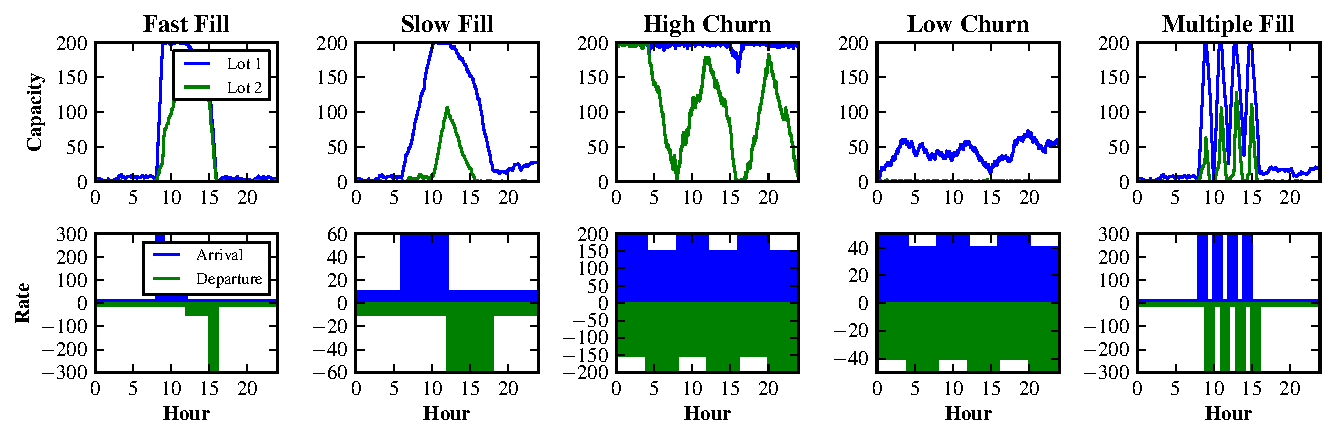
\includegraphics[width=\textwidth]{./simulator/figures/lots.pdf}

\caption{\textbf{Description of each type of lot simulated.} Five different
lots with different behaviors were used during simulations.}

\label{fig-lotsdescription}
\end{figure*}

\section{Evaluation}
\label{sec-evaluation}

We evaluated PocketParker in three ways. First, we conducted a controlled
experiment to determine the best parameter settings for our event detector.
Second, we implemented a parking lot simulator to experiment with various
kinds of lots under differing monitored fractions. Finally, we performed a
small-scale deployment of PocketParker on our campus and used it to monitor
two lots. Camera monitoring was used to ground truth the predictions from
our deployment dataset. Our evaluations confirm that PocketParker is
efficient and accurate.

\subsection{Detector Experiment}

\begin{figure}[t]
\centering
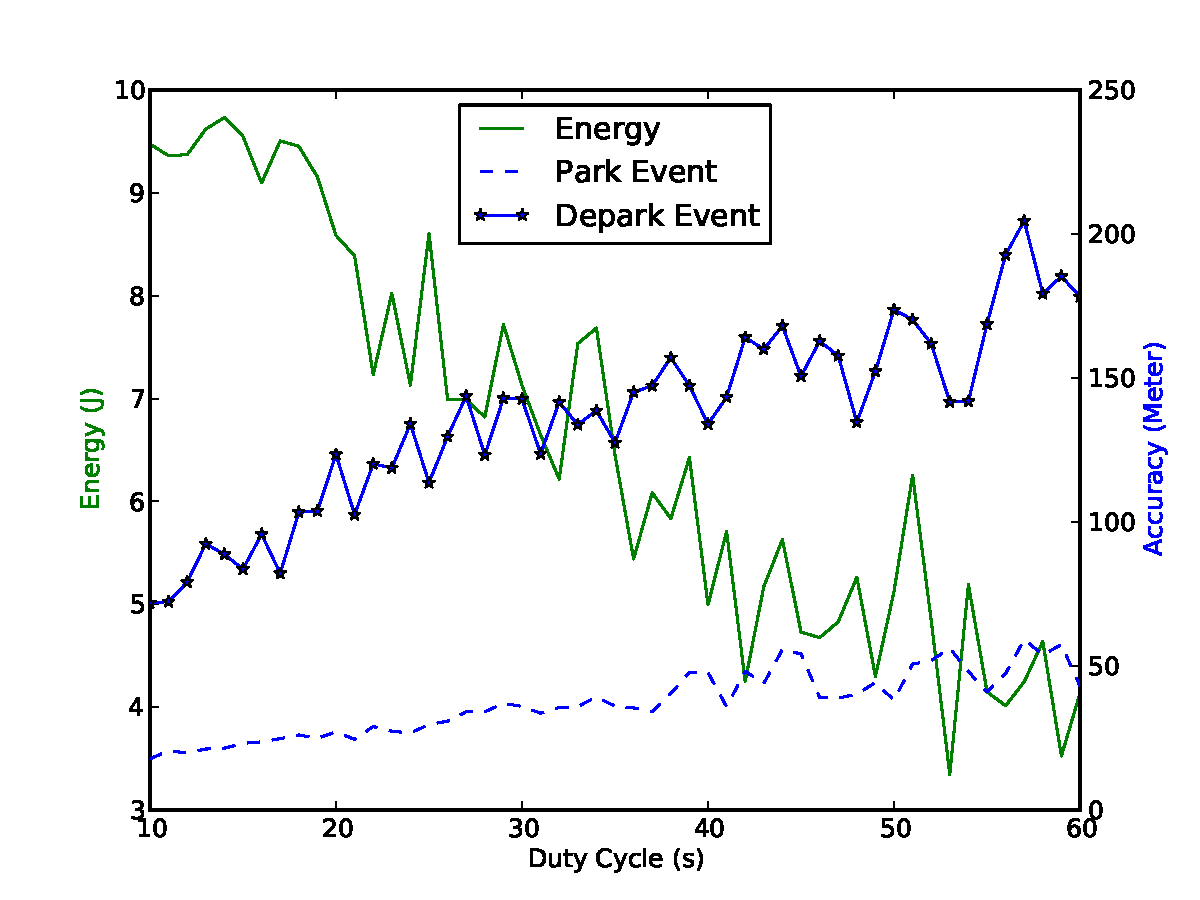
\includegraphics[width=3.325in]{./figures/Energy_accuracy.pdf}

\caption{\textbf{Power usage vs. detector accuracy.} Energy usage by
PocketParker is low at all duty cycles, so we chose a high duty cycle in
order to improve detection accuracy.}

\label{fig-energy}
\end{figure}

\newcolumntype{b}{>{\hsize=1.4\hsize}X}
\newcolumntype{s}{>{\hsize=.6\hsize}X}
\begin{table}[t]
{\small
\begin{threeparttable}
\begin{tabularx}{\columnwidth}{b s b s}
  {{\textbf{Carry Location}}} & {{\textbf{Count}}} &
  {{\textbf{Car Location}}} &
  {{\textbf{Count}}} \\
 \hline
In hand & 18 & Cup holder & 16 \\
Side bag & 10 & Car seat  & 9 \\
Back pack & 10 & Side bag & 10 \\
In hand talking & 7 & Back pack & 9 \\
Front pocket & 14 & Front pocket & 14 \\
Jacket pocket & 14 & Jacket pocket & 14 \\
Back pocket & 7 & Back pocket & 14 \\
\end{tabularx}
\end{threeparttable}
\caption{\textbf{Carry and car location for detector experiment.}
Eight participants generated 80 runs, carrying and placing the
phone in their car in many ways.}
\label{table-experiment}
}
\vspace*{-0.1in}
\end{table}


To determine the right parameter settings for our transition detector, we
conducted a controlled experiment. During this experiment, accelerometer and
GPS data was collected and stored continuously on each device, and
participants were asked to manually label each transition into and out of the
car. Afterwards, data was processed by a Python simulator implementing the
identical algorithm used by the PocketParker application, allowing us measure
accuracy and energy consumption as a function of the detector duty cycle.

Eight volunteers participated, including seven men and one woman. Seven were
right-handed and one was left-handed. Each was asked to conduct the same
experiment ten times: (1) carrying the instrumented phone, walk to their car;
(2) label departure; (3) drive around campus briefly; (4) park and label
arrival; (5) return inside. Since the way the phone is carried while walking
and placed in the car while driving affects the accelerometer readings, care
was taken to generate a good mix of carry and car location styles.
Table~\ref{table-experiment} shows the breakdown. The experiment permitted us
to obtain sensing data from a cross section of individuals possessing
different body morphologies, habits of driving cars, and ways of handling
mobile devices.

Figure~\ref{fig-energy} displays the tradeoff between energy usage and
detection accuracy as a function of the PocketParker duty cycle. Here we
combine an active period of 5s with a inactive period of variable length,
between 5~and~55s, for an overall duty cycle between 0.5 and 0.06. Our
simulator uses energy numbers from the Android Fuel Gauge application
o estimate average power consumption.  This graph measures the accuracy of
detected events in terms of distance from the actual location of the event
labeled by the participant.

As we expect, longer duty cycles consume less energy but produce longer
detection latencies which translate into higher distances from the event
location. Note also that the departure events have higher location error than
the parking events, because departing users are driving and therefore
traveling more rapidly. Overall power usage by PocketParker is low, under
10~mW at all duty cycles. Because PocketParker's ability to map parking
events into lots is affected by the detection distance accuracy, we chose a
low total period of 15~s for a 0.25 duty cycle. This allows PocketParker to
determine location to within 25~m for arrival events and 80~m for departures.
Power consumption at this duty cycle is 8~mW, representing 4.2\% of the
capacity of a 1500~mAh battery over 24~hours of usage.

\begin{figure}
\centering
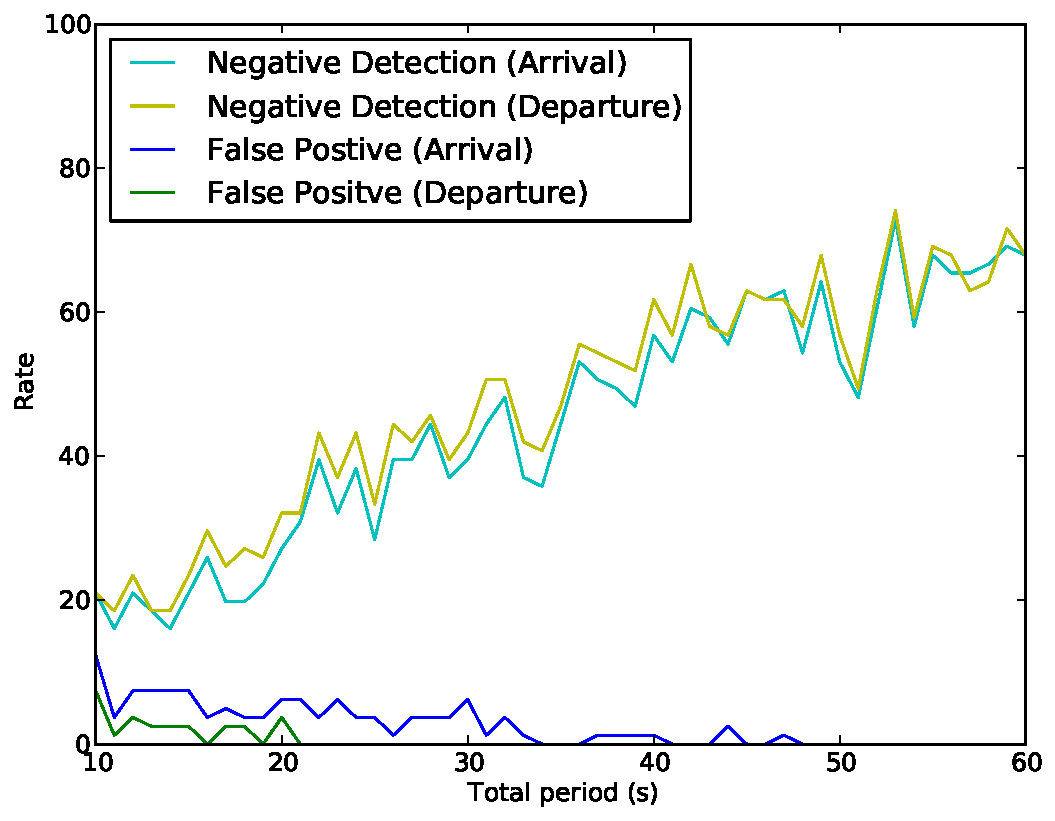
\includegraphics[width=3.325in]{./figures/Rate_FP_and_ND.pdf}

\caption{\textbf{False positive and negative rates as a function of detector
duty cycle.}} 

\label{fig-falsepositives}
\end{figure}

Using the same data we also examine the false positive and negative rates for
arrivals and departures. This is important since, without explicit user
input, it would be impossible to determine this information while
PocketParker is in use. Figure~\ref{fig-falsepositives} shows PocketParker
can detect 80\% of arrival and departure events correctly at the 0.25 duty
cycle we use. False positive rates are already quite low, and this is before
we apply our GPS availability filter and lot location filters. False
positives decline as the duty cycle decreases because PocketParker has fewer
opportunities to detect user activity.

\begin{figure}[t]
\centering
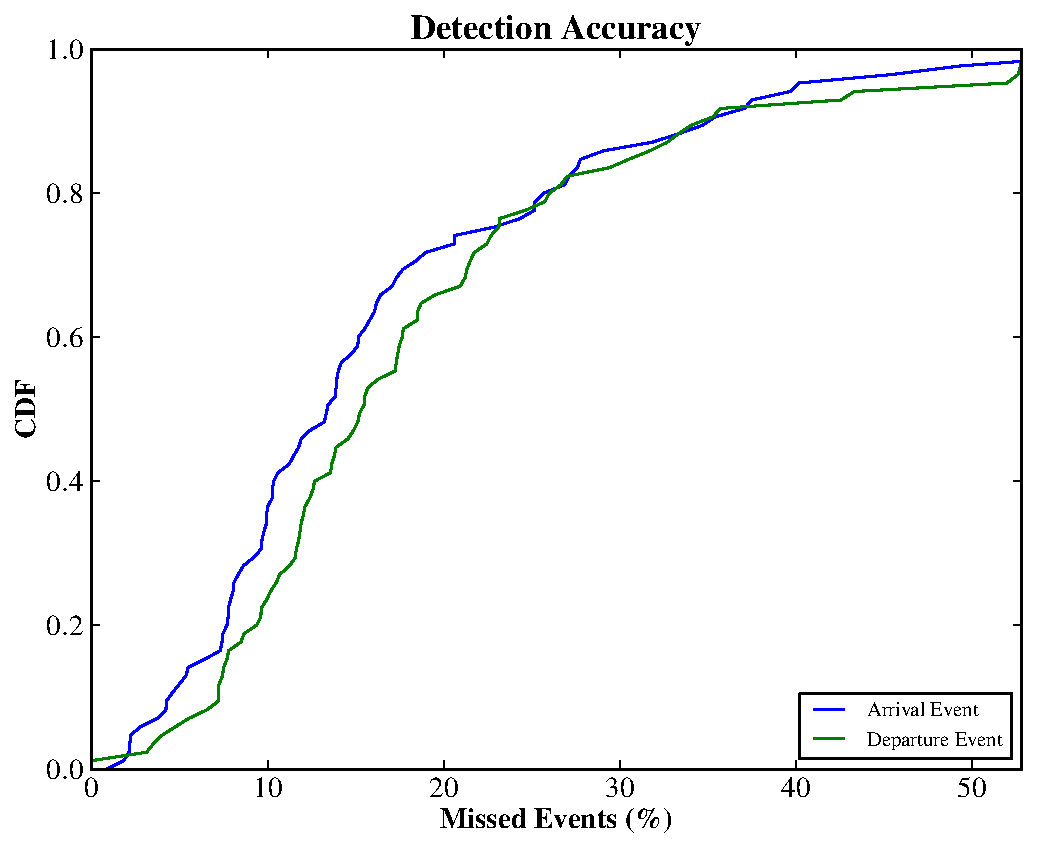
\includegraphics[width=3.325in]{./figures/MissedEvents_CDF.pdf}

\caption{\textbf{The percentage of missed parking Events.}}

\label{fig-missedevents}
\end{figure}

Figure~\ref{fig-missedevents} shows that PocketParker detects parking events 
faithfully: 80\% of users missed less than 25\% parking events. The main reason 
is because PocketParker has transition time threshold of 5 minutes. Therefore, 
PocketParker requires a minimum of 5 minutes to detect an user transition event
(from walking to driving or driving to walking). 

\subsection{Simulation Results}
\label{subsec-simulator}

To experiment with PocketParker in a more controlled setting, we implemented
a parking lot simulator in Python. Our simulator allows us to simulate any
number of parking lots associated with any number of points of interest with
varying desirability levels. For simplicity during our evaluation, we
simulate two lots 1~and~2 with lot~1 filling before lot~2, although lot
choice by simulated drivers is randomly weighted. Particularly for evaluating
our monitored fraction estimation, we use five types of lots that fill and
empty differently:

\begin{itemize}

\item \textbf{Fast Fill} and \textbf{Slow Fill} fill once per day quickly or
slowly, like a lot associated with a place of work.

\item \textbf{Multiple Fill} represents a lot that rapidly fills and empties
repeatedly during each day, like a campus lot or movie theater.

\item \textbf{High Churn} starts with lot~1 full and experiences continuously
high arrival and departures rates, like an airport parking lot.

\item \textbf{Low Churn} represents underutilized lots that never completely
fill, with lot~2 almost completely unused.

\end{itemize}

Figure~\ref{fig-lotsdescription} shows the arrival and departure rates for
each of the types of lot as well as the resulting per-lot capacity.

\begin{figure*}
\centering
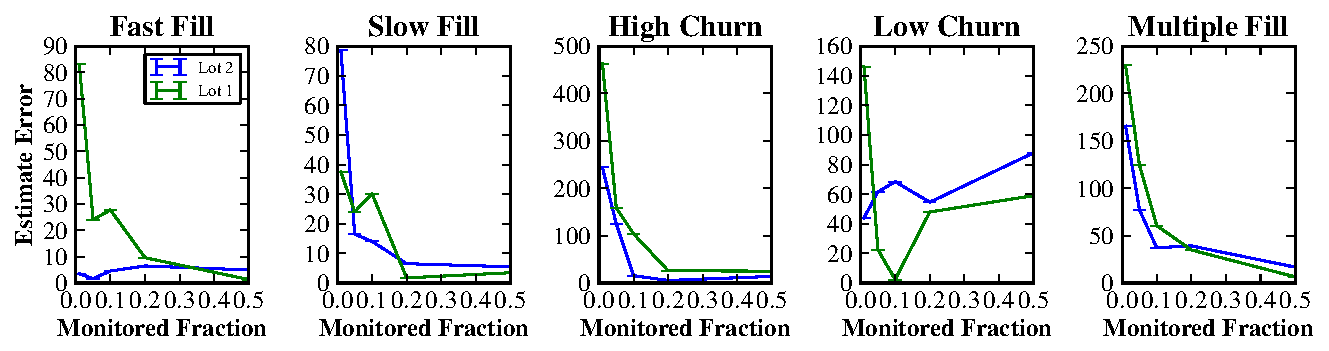
\includegraphics[width=\textwidth]{./simulator/figures/capacity_experiment.pdf}

\caption{\textbf{Errors in monitored fraction estimation.} Currently
PocketParker is better at estimating the monitored fraction when lots fill
and empty regularly.}

\label{fig-capacityerrors}
\end{figure*}

\subsubsection{Monitored fraction estimation}

In Section~\ref{subsubsec-monitored} we describe our approach to estimated
the monitored fraction, a parameter important to the operation of the
PocketParker availability estimator. Figure~\ref{fig-capacityerrors} shows
the results of 10 random simulations for each lot type. In each case, the
monitored fraction estimator uses a weeks worth of data and proceeds as
described previously. The error in the monitored fraction estimate is shown
as a function of the actual monitored fraction for the simulation used.

For the five types of lots, we would expect PocketParker to do better
monitored fraction estimation when lots fill regularly---Fast Fill, Slow
Fill, and Multiple Fill---and poorly when they do fill erratically or not at
all---High and Low Churn. The results in Figure~\ref{fig-capacityerrors}
generally follow this pattern. Errors for High Churn are quite high, and Low
Churn errors persist even at high monitored driver fractions. This is
natural, as the Low Churn lot never fills.  By contrast, the accuracy rate for
the Fast, Slow and Multiple Fill models improve with an increasing fraction of
monitored drivers.

\begin{figure}[t]
\centering
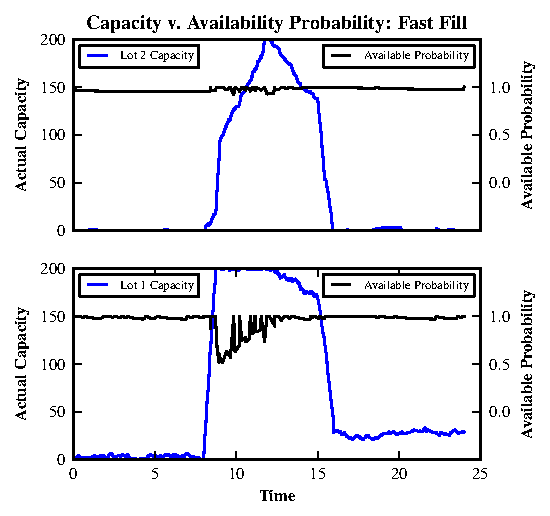
\includegraphics[width=3.325in]{./simulator/figures/tracking_fastfill.pdf}

\caption{\textbf{Availability probabilities tracking lot capacity.} Dips in
the availability probability correspond to times when PocketParker believes
the lot is full. Discontinuities are caused by departures, which set the
instantaneous probability that the lot is available to 1.0.}

\label{fig-trackingexample}
\end{figure}

\subsubsection{Probability and availability}

At this point we take a closer look at the way that PocketParker adjusts lot
availability probabilities. Keep in mind that the absolute value of the
availability probability for each lot may not meaningful. Instead,
PocketParker uses the probabilities to order available lots in response to
queries. We examine its accuracy at performing this essential task next.
However, it is illustrative to examine the probabilities PocketParker
maintains and observe how they vary as the number of available spots in the
lot changes.

Figure~\ref{fig-trackingexample} shows a 24~hour simulation of a Fast Fill
parking lot with a monitored fraction of 0.1 and a 10\% error in the
estimation of the monitored fraction. The ground truth capacity of the lot as
simulated is plotted next to the PocketParker probability that the lot has an
available spot. At the beginning of the simulation, both lots are marked as
free. When lot~1 fills and lot~2 begins to fill, generating implicit searches
in lot~1, the availability probability of lot~1 drops. It spikes upward
repeatedly due to departures from lot~1---which reset the short-term
probability of an available spot back to 1---but does not equal the
probability for lot~2 again until the point when the departure rate for lot~1
climbs.

\subsubsection{Prediction accuracy}

\begin{table}[t]
\begin{threeparttable}
{\small
\begin{tabularx}{\columnwidth}{Xrrrrr}
\multicolumn{1}{c}{\textbf{Type}} & 
\multicolumn{1}{c}{\textbf{$f_m$}} & 
\multicolumn{1}{c}{\textbf{$f_m$ Error}} & 
\multicolumn{1}{c}{\textbf{Correct}} & 
\multicolumn{1}{c}{\textbf{Missed}} & 
\multicolumn{1}{c}{\textbf{Waste}}\\ \toprule

\textbf{Campus} & & & & & \\
\midrule
& 0.20 & 0.10 & 100.0 \% & 0.0 \% & 0.0 \% \\
\textbf{Fast Fill} & & & & & \\
\midrule
& 0.01 & 0.10 & 75.1 \% & 24.7 \% & 0.2 \% \\
& 0.05 & 0.10 & 72.3 \% & 26.2 \% & 1.5 \% \\
& 0.10 & 0.10 & 80.0 \% & 15.6 \% & 4.4 \% \\
& 0.10 & 0.20 & 86.6 \% & 11.2 \% & 2.2 \% \\
& 0.10 & 0.50 & 89.7 \% & 7.7 \% & 2.7 \% \\
& 0.10 & 1.00 & 93.0 \% & 4.8 \% & 2.2 \% \\
& 0.20 & 0.10 & 87.9 \% & 8.5 \% & 3.6 \% \\
& 0.50 & 0.10 & 94.0 \% & 5.0 \% & 1.0 \% \\
\textbf{High Churn} & & & & & \\
\midrule
& 0.01 & 0.10 & 54.0 \% & 0.0 \% & 46.0 \% \\
& 0.05 & 0.10 & 55.3 \% & 0.0 \% & 44.7 \% \\
& 0.10 & 0.10 & 63.6 \% & 0.0 \% & 36.4 \% \\
& 0.10 & 0.20 & 62.2 \% & 0.0 \% & 37.8 \% \\
& 0.10 & 0.50 & 60.1 \% & 0.0 \% & 39.9 \% \\
& 0.10 & 1.00 & 61.8 \% & 0.0 \% & 38.2 \% \\
& 0.20 & 0.10 & 64.0 \% & 0.0 \% & 36.0 \% \\
& 0.50 & 0.10 & 70.6 \% & 0.0 \% & 29.4 \% \\
\textbf{Low Churn} & & & & & \\
\midrule
& 0.01 & 0.10 & 98.4 \% & 0.0 \% & 1.6 \% \\
& 0.05 & 0.10 & 89.1 \% & 0.0 \% & 10.9 \% \\
& 0.10 & 0.10 & 94.1 \% & 0.0 \% & 5.9 \% \\
& 0.10 & 0.20 & 91.0 \% & 0.0 \% & 9.0 \% \\
& 0.10 & 0.50 & 87.9 \% & 0.0 \% & 12.1 \% \\
& 0.10 & 1.00 & 87.8 \% & 0.0 \% & 12.2 \% \\
& 0.20 & 0.10 & 92.5 \% & 0.0 \% & 7.5 \% \\
& 0.50 & 0.10 & 91.6 \% & 0.0 \% & 8.4 \% \\
\textbf{Multiple Fill} & & & & & \\
\midrule
& 0.01 & 0.10 & 51.4 \% & 42.8 \% & 5.8 \% \\
& 0.05 & 0.10 & 71.2 \% & 26.0 \% & 2.9 \% \\
& 0.10 & 0.10 & 85.2 \% & 13.2 \% & 1.6 \% \\
& 0.10 & 0.20 & 79.4 \% & 17.5 \% & 3.1 \% \\
& 0.10 & 0.50 & 86.2 \% & 12.7 \% & 1.1 \% \\
& 0.10 & 1.00 & 77.6 \% & 20.9 \% & 1.5 \% \\
& 0.20 & 0.10 & 92.1 \% & 7.5 \% & 0.5 \% \\
& 0.50 & 0.10 & 91.6 \% & 7.8 \% & 0.6 \% \\
\textbf{Slow Fill} & & & & & \\
\midrule
& 0.01 & 0.10 & 70.7 \% & 26.0 \% & 3.2 \% \\
& 0.05 & 0.10 & 78.8 \% & 17.5 \% & 3.7 \% \\
& 0.10 & 0.10 & 82.1 \% & 13.3 \% & 4.6 \% \\
& 0.10 & 0.20 & 75.4 \% & 15.2 \% & 9.4 \% \\
& 0.10 & 0.50 & 80.5 \% & 19.3 \% & 0.2 \% \\
& 0.10 & 1.00 & 85.2 \% & 12.5 \% & 2.3 \% \\
& 0.20 & 0.10 & 87.8 \% & 9.8 \% & 2.4 \% \\
& 0.50 & 0.10 & 93.8 \% & 5.6 \% & 0.6 \% \\
\end{tabularx}
}
\caption{\textbf{Accuracy of PocketParker predictions for various kinds of lots and parameters.}}
\label{table-accuracy}
\end{threeparttable}
\end{table}



PocketParker exists to help drivers choose parking lots efficiently. Here,
we examine the accuracy of the predicitions generated by our system. To do
so, we have PocketParker rank two model lots in order of preference at
regular timesteps.  We compare these results with the ground truth available
through a simulator and then categorize them as be in a correct prediction,
a missed opportunity, or a waste of time. A missed opportunity represents a
case where a more desirable lot was available than the one that PocketParker
recommended. A waste of time indicates that PocketParker sent the user to a
lot that did not actually have an available spot. Table~\ref{table-accuracy}
shows data results from simulations run using varying monitored
fractions$f_m$ of drivers.

\begin{figure}[t]
\centering
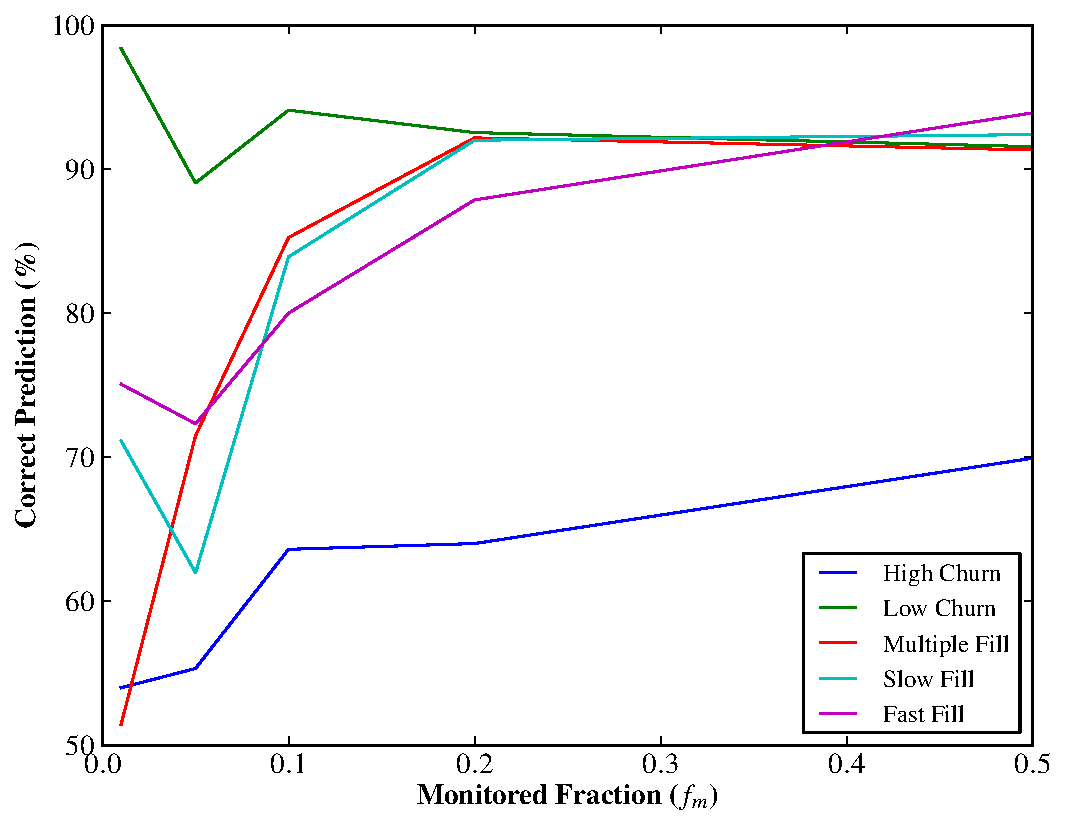
\includegraphics[width=3.325in]{./simulator/figures/accuracy_graph.pdf}

\caption{\textbf{Accuracy predictions for various kind of lots and parameters.}}
\label{fig-accuracy}
\end{figure}

Also, Figure~\ref{fig-accuracy} shows that several trends can be observed 
in the results. First, overall PocketParker does well on most lot types. 
The High Churn lot presents the greatest difficulty, which we would expect 
since its large number of incoming and outgoing drivers make prediction 
difficult. We are also concerned that the High Churn errors are largely 
waste of time errors, indicating that PocketParker is frequently sending 
drivers to the wrong lot.  This is likely because it is predicting that 
spots are available longer than they actually are. Clearly more work is 
needed to determine the right approach for High Churn lots.

Excluding the High Churn lot, the lot with the lowest correct percentage with
a $f_m > 0.1$ is 80\% for the Slow Fill lot.  Accuracy for all lots above
this $f_m$ is consistently good for all lots save the High Churn model.  The
Low Churn lot does have a small number of errors but this is because both lots
are usually empty.

One unavoidable lower bound to the accuracy of PocketParker is imposed by the
frequency of parking events.  This is because PocketParker has the most
information about lot availability during active periods of arrival and
departure events. Once it stops receiving event information, prediction
uncertainty grows.  Thus, to the degree that PocketParker queries follow at
least pattern of arrivals and departures, we will have fresh data and do well.

\subsection{Deployment}

\begin{figure*}
\centering
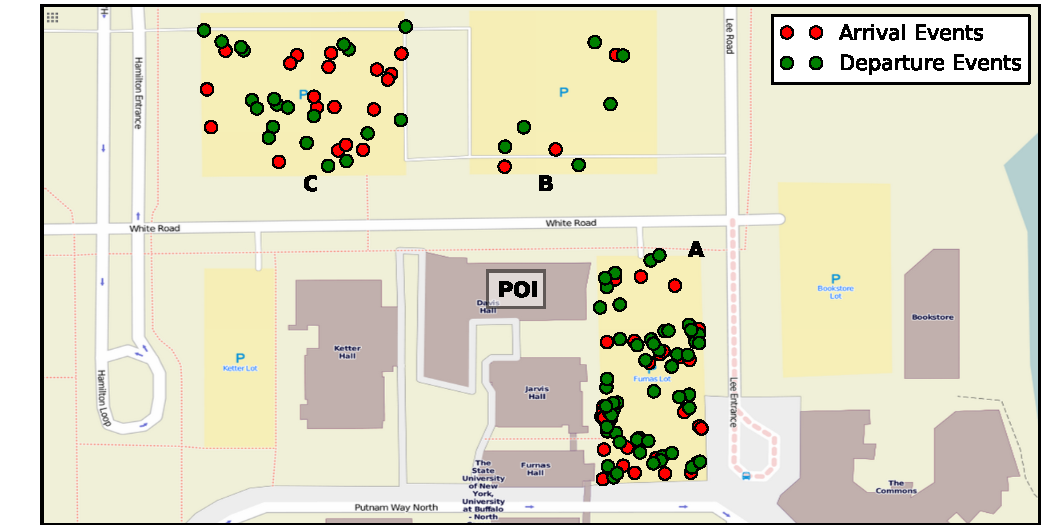
\includegraphics[width=\textwidth]{./figures/EventsOnThreeParkingLot.pdf}

\caption{\textbf{Map showing 217~parking events detected by PocketParker
during our forty-five-day deployment in three key lots.}  These were
generated by 26 participants.  Lot~A is considered the most desirable of the
three lots, a fact reflected in the higher event density of this lot.  
Lots~A~and~B were monitored by cameras to establish ground truth}

\label{fig-events}
\end{figure*}

Finally, to establish the accuracy of PocketParker we performed a pair of
deployments on our university campus.  The system structure was the same in
both cases:  The only infrastructure required was the PocketParker server for
receiving events and generating availability estimates.  For the first
rollout, we installed the PocketParker client on the Android version 4.1
system and the Samsung Nexus~S~4G smartphone.  In this experiment, we
configured PocketParker to operate in the background and to require no user
interaction.   We recruited five participants who generated 372 events over
ten days---202 arrivals and 170 departures.

In our second rollout, we deployed PocketParker on the Android version 4.2
system and Galaxy Nexus smartphone.  PocketParker, rather than running in the
background, displayed to users a campus map showing recent parking events.
The userbase involved 105 total participants, 102 of whom were members of
PhoneLab, an existing campus mobile phone network.  Over 45 days of 
monitoring, they generated 10,827 events -- 5916 arrivals and 4911 
departures -- for an average of 241 per day.  Our main and medical 
campuses produced 3645 and 846 total events respectively, with non-campus 
locales contributing the remaining 6336 events.

Figure~\ref{fig-events} shows all of the events that occurred in three key
lots that we monitored in the second experiment. Our computer science
building is labeled as the point of interest (POI). To determine ground
truth availability, we positioned four cameras at locations within the
building to monitor lots A~and~B in Figure~\ref{fig-events}.  Despite the fact
that many parking events took place in lot~C, we were unable to locate a
suitable unobstructed vantage point to gather camera data for that lot.
Nexus~S~4G smartphones equipped with fish-eye lenses served as our cameras.
Each took time lapse images at 1~Hz, time-stamped them using NTP and uploaded
them to a central server. A total of 34,138 images were collected for the two 
monitored lots over two weeks.

To measure capacity, we hand-coded four days' worth of images for two lots on
a ten-point scale at ten-minute intervals. We were particularly interested
in the transition between empty and full states, so we were careful to ensure
that the lot was never marked completely full if there was a single available
spot visible. We generate 4 different dataset using parking events in 
camera-monitored lots A~and~B and then feed the events into the PocketParker
estimation engine.

Table~\ref{table-accuracy} also includes numbers for our campus deployment
labeled as ``Campus''. Overall the accuracy of PocketParker is excellent, 
achieving 94.2\% accuracy at a monitored driver fraction of 0.2. 
